\section{Classifier Evaluation}
\subsection{Confusion Matrix}
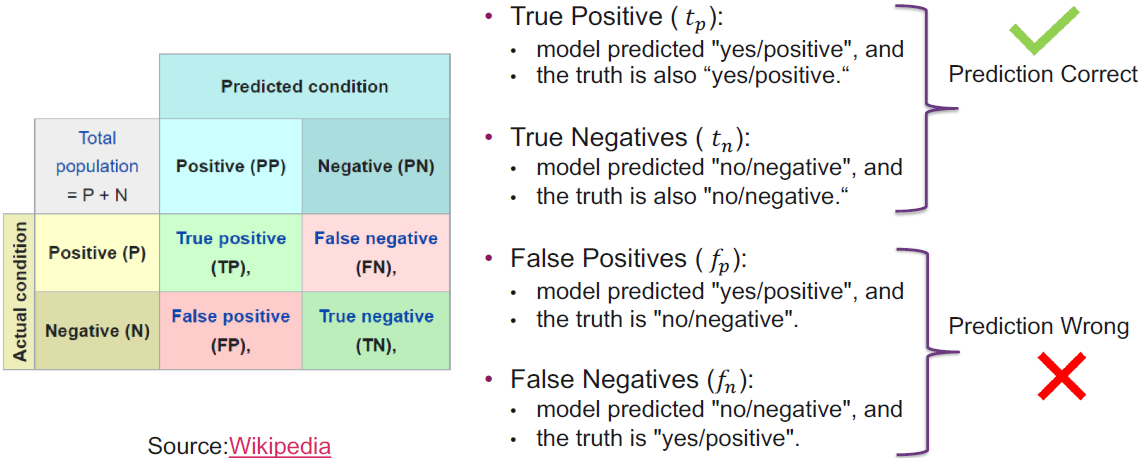
\includegraphics[width=\linewidth]{./img/confusion_matrix.png}
\textbf{Mean Accuracy:}
\begin{itemize}
    \item How often is the classifier correct?
    \item $A = (t_p + t_n) / n$
\end{itemize}
\textbf{Mean Error:}
\begin{itemize}
    \item How often is the classifier wrong?
    \item $E = (f_p + f_n) / n$
\end{itemize}
\textbf{Precision:}
\begin{itemize}
    \item When the prediction is 1, how often is it correct (True Positive)?
    \item $P = t_p / (t_p + f_p)$
\end{itemize}
\textbf{Sensitivity, Recall, True Positive Rate (TPR):}
\begin{itemize}
    \item How often the prediction is 1 when it's actually 1 (True Positive)
    \item $R = t_p / (t_p + f_n)$
\end{itemize}
\textbf{Miss Rate, False Negative Rate (FNR)}
\begin{itemize}
    \item $MR = 1 - TPR$
\end{itemize}
\textbf{Miss Rate, False Positive Rate (FPR)}
\begin{itemize}
    \item $R = f_p / (f_p + t_n)$
\end{itemize}

\subsection{Why Accuracy is not enough?}
\begin{itemize}
    \item If the prediction is constant the accuracy may still look decent
    \item E.g. always predict false
    \item 90\% of the data is false
    \item Accuracy = 90\% (decent)
    \item Precision = 0
    \item Recall = 0
\end{itemize}

\subsection{Precision vs. Recall}
\begin{itemize}
    \item Increasing precision reduces Recall and vice versa
    \item Threshold is a business decision (depending on goals)
\end{itemize}

\subsection{Receiver Operating Characteristics (ROC Curve)}
\begin{itemize}
    \item Defined by FPR and TPR as x and y axes
    \item Visualizes tradeoff between TPR (benefits) and FPR (cost)
\end{itemize}
\begin{center}
    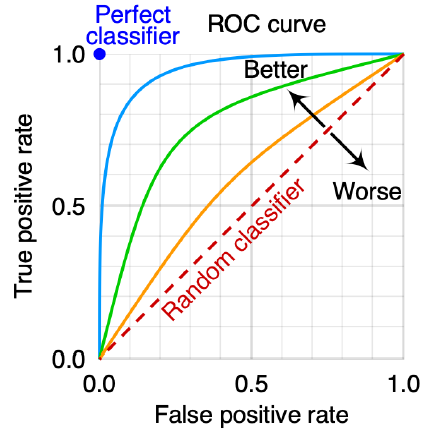
\includegraphics[width=0.4\linewidth]{./img/roc.png}
\end{center}
\textbf{Area under the curve}
\begin{itemize}
    \item Area under the ROC curve
    \item Shows how well the TPR and FPR is looking in the aggregate
    \item The greater the area under the curve, the higher the quality of the model
    \item The greater the area, the higher the ratio of TP to FP
\end{itemize}

\section{KNN}

\subsection{Linear Seperability (Decision Boundary)}
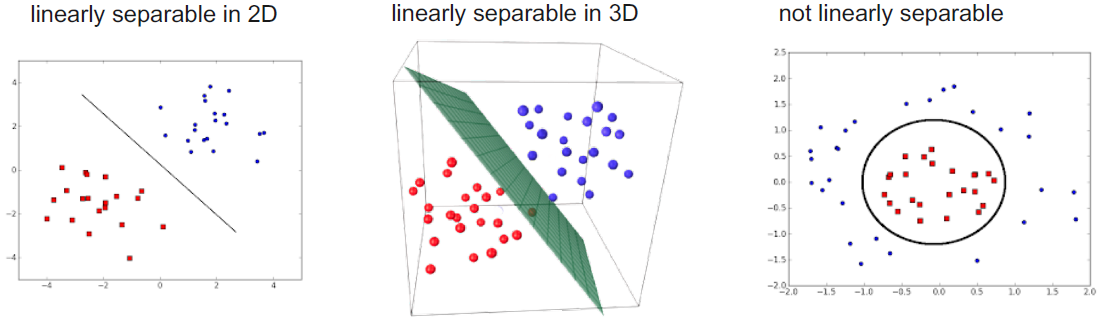
\includegraphics[width=1\linewidth]{./img/linear_sep.png}

\begin{itemize}
    \item Based on logistic regression model, you can draw a line
    \item This is the Linear decision boundary
    \item If a simple line perfectly seperates the classes, then the classes are said to be linearely seperable
\end{itemize}

\subsection{Non-Linear decision boundary}
\begin{itemize}
    \item When classes are not linearly seperable
    \item Resort to polynomial terms
\end{itemize}

\subsection{Multi-class classification}
\begin{itemize}
    \item e.g. COVID-Varianten, Weather-classes (sunny, cloudy, stormy..)
    \item Logistic Regresion can be extended One-vs-Rest (Cat/NoCat) / One-vs-One (Cat/Dog..)
    \item ...but slow training and can result in ambiguity. Therefore maybe KNN works better
\end{itemize}

\subsection{k-Neares Neighbors (KNN)}
\begin{itemize}
    \item super simple way to classify data (\textit{supervised learning})
    \item Works well for multi-class classification
    \item no complex training necessary, all data is used for each classification
    \item Basic Idea: A datapoint is know by the company it keeps
    \item Choose $k$ and compute distance to every neighbour for every datapoint
    \item Returns the most frequent class of the $k$ nearest neighbours\\
\end{itemize}
\textbf{Ablauf}
\begin{enumerate}
    \item Start with a dataset with known categories
    \item Add a new Datapoint or cell, with unknown category, to the cluster. We don't know this Datapoint's category because it was taken from another dataset where the Datapoints were not properly sorted
    \item We classify the new Datapoint by looking at the nearest annotated cells ("nearest neighbor)
    \begin{enumerate}
        \item If the \textit{k} in \textit{k-nearest neighbors} is equal to 1, then we only use the nearest neighbor to define the category
    \end{enumerate}
\end{enumerate}
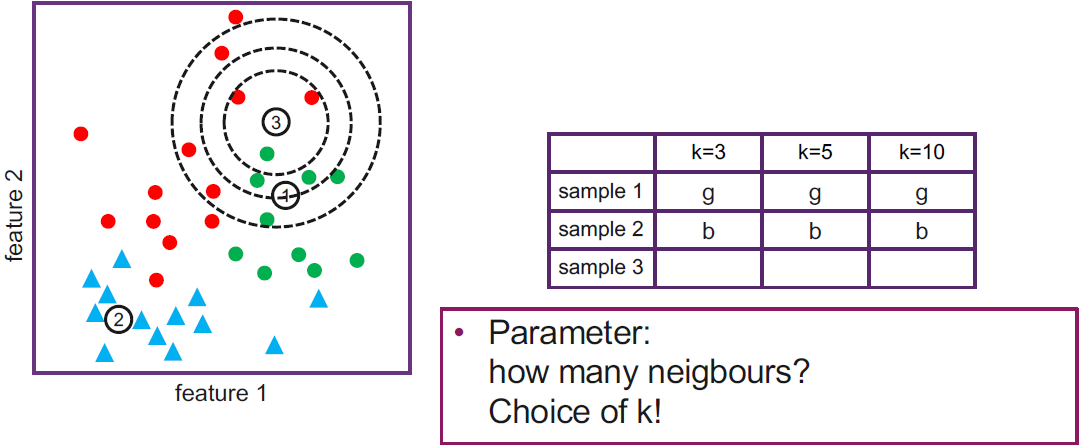
\includegraphics[width=0.8\linewidth]{./img/knn.png}
\subsubsection{Distance Metric}
\begin{itemize}
    \item Cosine Distance (Winkel)
    \begin{itemize}
        \item $\cos(\theta)=\frac{x_1 \cdot x_2}{|x_1| \cdot |x_2|}$
    \end{itemize}
    \item Manhattan Distance (Rhombus)
    \begin{itemize}
        \item $d_M=\displaystyle\sum_{i=1}^n | x_{1,n}-x_{2,n}|$
    \end{itemize}
    \item Euclidean Distance (most used, Kreis)
    \begin{itemize}
        \item $d_E=\sqrt{\displaystyle\sum_{i=1}^n(x_{1,n}-x_{2,n})^2}$
    \end{itemize}
    \item Minkowski Distance
\end{itemize}

\subsubsection{Choose of k}
\begin{itemize}
    \item if k is small, risk of overfitting (the decision boundary is dominated by only 1 datapoint)
    \item if k is big, risk of underfitting (decision boundaries are very smooth and cannot capture small differences that occur at the boundaries. Edge-cases are more likely to be misclassified)
    \item use confusion matrix the evaluate best k (e.g. precision and recall)
\end{itemize}

\subsubsection{Advantages}
\begin{itemize}
    \item Easy and simple ML model
    \begin{itemize}
        \item almost no training cost, but more calculating distance when used costs
    \end{itemize}
    \item Few hyperparameters to tune
\end{itemize}

\subsubsection{Disadvantages}
\begin{itemize}
    \item $k$ should be wisely selected (e.g. use cross-validation)
    \item Large computation cost during runtime if sample size is large
    \item Not efficient for high dimensional datasets
    \item Proper scaling should be provided for fair treatment among features
\end{itemize}

\subsubsection{Hyperparameters}
\begin{itemize}
    \item \textbf{K Value}: how many neighbours to participate in the KNN algo. If $k$ is to small = \textbf{overfitting} (fitting the noise) / if $k$ ist to large = \textbf{undefitting} (edge-casese more likely to be misclassified)
    \item \textbf{Distance Function}: Euclidean distance is most used
\end{itemize}

\subsection{Excercise}
\begin{minted}{python}
KNNclf = KNeighborsClassifier(n_neighbors=5, metric='euclidean')
KNNclf.fit(X_train, Y_train)
Y_hat = KNNclf.predict(X_test)
\end{minted}
\begin{itemize}
    \item For each different $k$, calculate accuracy, precision $tp/(tp+fp)$ and recall $tp/(tp+fn)$
    \item Which value of k would be your choose?
\end{itemize}